\documentclass[12pt, twoside]{article}
\usepackage[letterpaper, margin=1in, headsep=0.5in]{geometry}
\usepackage[english]{babel}
\usepackage[utf8]{inputenc}
\usepackage{amsmath}
\usepackage{amsfonts}
\usepackage{amssymb}
\usepackage{tikz}
\usetikzlibrary{quotes, angles}
\usepackage{graphicx}
\usepackage{multicol}

%\usepackage{pgfplots}
%\pgfplotsset{width=10cm,compat=1.9}
%\usepgfplotslibrary{statistics}
%\usepackage{pgfplotstable}
%\usepackage{tkz-fct}
%\usepackage{venndiagram}

\usepackage{fancyhdr}
\pagestyle{fancy}
\fancyhf{}
\renewcommand{\headrulewidth}{0pt} % disable the underline of the header

\fancyhead[RE]{\thepage}
\fancyhead[RO]{\thepage \\ Name: \hspace{3cm}}
\fancyhead[L]{BECA / Dr. Huson / Geometry 10th Grade\\* Unit 1: Introduction to Geometry\\20 September 2019}

\begin{document}
\subsubsection*{2.5 Homework: Area, perimeter, line segments}
  \vspace{0.25cm}
  \begin{enumerate}

\item Given the rectangle $ABCD$ shown below, with $AB=9.1$ and $BC=4.3$. Find the area of the rectangle.
\begin{flushleft}
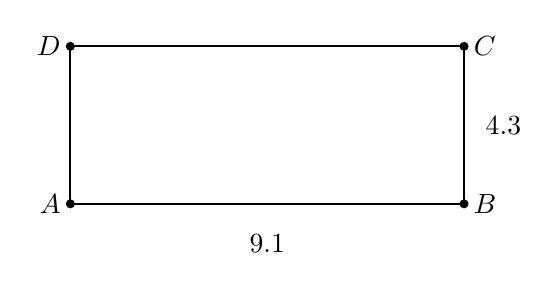
\begin{tikzpicture}
  \draw [-, thick] (0,0)--(5,0)--(5,2)--(0,2)--cycle;
  \draw [fill] (0,0) circle [radius=0.05] node[left]{$A$};
  \draw [fill] (5,0) circle [radius=0.05] node[right]{$B$};
  \draw [fill] (5,2) circle [radius=0.05] node[right]{$C$};
  \draw [fill] (0,2) circle [radius=0.05] node[left]{$D$};
  \node at (5.5, 1){4.3};
  \node at (2.5, -0.5){9.1};
\end{tikzpicture}
\end{flushleft} \vspace{1cm}  

\item The rectangle $MATH$ has an area of 102, with length $MA=12$. Find the width of the rectangle $AT$.
\begin{flushleft}
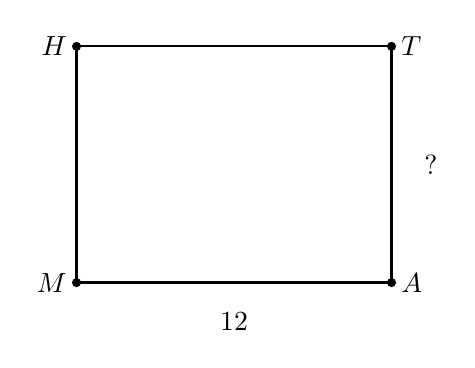
\begin{tikzpicture}
  \draw [-, thick] (0,0)--(4,0)--(4,3)--(0,3)--cycle;
  \draw [fill] (0,0) circle [radius=0.05] node[left]{$M$};
  \draw [fill] (4,0) circle [radius=0.05] node[right]{$A$};
  \draw [fill] (4,3) circle [radius=0.05] node[right]{$T$};
  \draw [fill] (0,3) circle [radius=0.05] node[left]{$H$};
  \node at (4.5, 1.5){?};
  \node at (2, -0.5){12};
\end{tikzpicture}
\end{flushleft} \vspace{2cm}  

\item Find the area of $\triangle ABC$. The altitude $h$ of the triangle is 3.15 centimeters and the base $AB=7.8$ cm.\\[0.5cm]
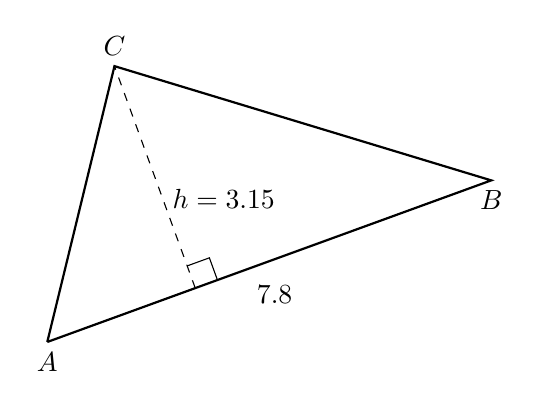
\begin{tikzpicture}[scale=1, rotate=20]
  \draw [thick]
    (2,0)node[below]{$A$}--
    (8,0)node[below]{$B$}--
    (4,3)node[above]{$C$} --(2,0);
 \draw [dashed] (4,0)--(4,3);
 \draw (4,0)++(0.3,0)--++(0,0.3)--+(-0.3,0);
 \node at (4,1.2)[right]{$h=3.15$};
 \node at (5,-0.2)[below]{$7.8$};
\end{tikzpicture} \vspace{1.0cm}

\newpage

\item One side of the $\triangle ABC$ has a length $AB=8$. The triangle's area is 44. Find the length of the altitude $h$ of the triangle to vertex $C$ and perpendicular to side $\overline{AB}$.\\[0.5cm]
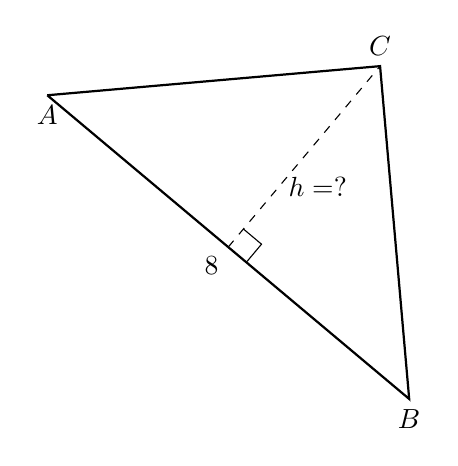
\begin{tikzpicture}[scale=1, rotate=-40]
  \draw [thick]
    (2,0)node[below]{$A$}--
    (8,0)node[below]{$B$}--
    (5,3)node[above]{$C$} --(2,0);
 \draw [dashed] (5,0)--(5,3);
 \draw (5,0)++(0.3,0)--++(0,0.3)--+(-0.3,0);
 \node at (5,1)[right]{$h=?$};
 \node at (5,0)[below left]{$8$};
\end{tikzpicture} \vspace{1.0cm}


  \item Given $\overleftrightarrow{RS}$ as shown on the number line, with $R=-1.0$ and $S=5.6$. \\[20pt] % Midpoint
  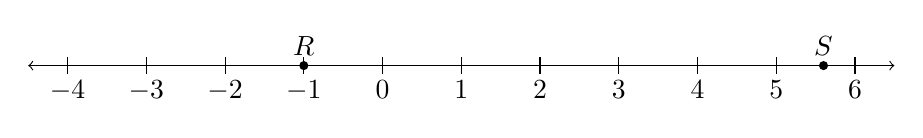
\begin{tikzpicture}
    \draw [<->] (-4.5,0)--(6.5,0);
    \foreach \x in {-4,...,6} %2 leading for diff!=1
      \draw[shift={(\x,0)},color=black] (0pt,-3pt) -- (0pt,3pt) node[below=5pt]  {$\x$};
      \draw [fill] (-1.0,0) circle [radius=0.05] node[above] {$R$};
      \draw [fill] (5.6,0) circle [radius=0.05] node[above] {$S$};
  \end{tikzpicture}
  \begin{enumerate}
    \item What is the exact distance on the number line between the points $R$ and $S$? \vspace{3cm} 
    \item The points $T$ and $U$ trisect $\overline{RS}$. Find the values of $T$ and $U$, and mark and label them on the numberline $\overleftrightarrow{RS}$. 
  \end{enumerate} \vspace{3cm}  
  
  \newpage

  \item Given $\overline{ABC}$, $AB=\frac{2}{3}$, and $AC=3 \frac{1}{3}$.\\ [0.5cm]
  Find ${BC}$.\\[1.5cm]
      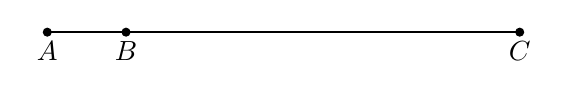
\begin{tikzpicture}
        \draw [-, thick] (1,0)--(7,0);
        \draw [fill] (1,0) circle [radius=0.05] node[below]{$A$};
        \draw [fill] (2,0) circle [radius=0.05] node[below]{$B$};
        \draw [fill] (7,0) circle [radius=0.05] node[below]{$C$};
      \end{tikzpicture}\\[1.5cm]
      The postulate used in this problem is the \rule{6cm}{0.15mm}.
      \vspace{1.5cm}

  \item Given the diagram shown below. \vspace{0.25cm}
  \begin{enumerate}
    \item  Measure the angle $AEB$. $m \angle AEB = $ \rule{4cm}{0.15mm} \bigskip
    \item Name an angle that is supplementary to $\angle DEB$: \rule{4cm}{0.15mm} \bigskip
    \item Name a pair of opposite rays: \rule{4cm}{0.15mm}
  \end{enumerate}
  \vspace{1cm}
  \begin{center}
  \begin{tikzpicture}[scale=1.3, rotate=-30]
    \draw [->, thick] (0,0)--(50:6);
    \draw [<->, thick] (-6,0)--(5,0);
    \draw [->, thick] (0,0)--(0,3);
    \draw (0,0)++(0.3,0)--++(0,0.3)--+(-0.3,0);
    %\draw [fill] (-1,2.5) circle [radius=0.05] node[left ]{$B$};
    \draw [fill] (50:4) circle [radius=0.05] node[below right]{$B$};
    \draw [fill] (-4,0) circle [radius=0.05] node[below]{$A$};
    \draw [fill] (0,0) circle [radius=0.05] node[below left]{$E$};
    \draw [fill] (0,2) circle [radius=0.05] node[left]{$C$};
    \draw [fill] (4,0) circle [radius=0.05] node[below]{$D$};
  \end{tikzpicture}
  \end{center}
  
   \newpage 

   \item Find the perimeter $P$ of the shape shown below, given the side lengths marked (not drawn to scale). All angles are $90^\circ$. Completely mark the diagram with the two missing lengths and show an equation for $P$ as a sum of each side's length.
   \vspace{1cm} 
   \begin{flushleft}
   \begin{tikzpicture}
     \draw [-, thick] (0,0)--(5,0)--(5,2)--(3,2)--(3,3)--(0,3)--cycle;
     %\draw [fill] (0,0) circle [radius=0.05] node[left]{$A$};
     %\draw [fill] (7,0) circle [radius=0.05] node[right]{$B$};
     %\draw [fill] (7,2) circle [radius=0.05] node[right]{$C$};
     %\draw [fill] (0,2) circle [radius=0.05] node[left]{$D$};
     \node at (5.5, 1){5};
     \node at (1.5, 3.5){7};
     \node at (2.5, -0.5){12};
     \node at (-0.5, 1.5){7};
   \end{tikzpicture}
   \end{flushleft} \vspace{2cm}

   \item Given the collinear points $P$, $Q$, and $R$, with $PQ=4x+4$, $QR=2x+2$, and $PR=5x+12$. Find ${PQ}$.\\*[5pt]
   Complete all steps for full credit: the drawing to the top right, an equation and solution for $x$ on the left, followed by the answer to the question. Write the check to the bottom right.
\vspace{4cm}

  \end{enumerate}
\end{document}
